\section{Federated Learning}
% Introduce federated learning
Many modern machine learning algorithms require large volumes of diverse data to achieve optimal performance. Real-world data is often distributed among multiple nodes that are unable to share it with each other due to privacy regulations such as GDPR \cite{gdpr}, reducing the amount of data available to train models on and negatively impacting trained performance \cite{data_volume}. Federated Learning (FL) \cite{survey_on_fed_learning} is a technique in machine learning that aims to train a single model using all available data across nodes without requiring any data to be shared among them. \\

% Intro on how fed learning works and different types
There are a multitude of published FL frameworks \cite{fed_table_survey}, each with different merits and drawbacks for certain use cases. Federated Averaging (FedAvg) \cite{fed_learning} is a commonly used yet simple framework, which splits training into iterations where three steps take place:
\begin{enumerate}
	\item A copy of the current model is sent to each node from the central server
	\item Each node performs some training with their copy of the model and their own private data
	\item The trained models from each node are sent back to the server to aggregate into the new server model
\end{enumerate}
The server model improves over time, and after a certain number of steps, the training is complete and the server model is the final output. \\

% Specify why federated learning is better than conventional learning
As it does not require data to be shared between nodes, FL is naturally beneficial for privacy sensitive tasks compared to conventional machine learning where the data is aggregated in a central location \citeme. Additionally, as FL performs training on multiple nodes in parallel, it can make better use of available training resources in situations where processing power is distributed among multiple nodes \citeme.

% federate distributed
One branch of FL is distributed federated learning (DFL). This algorithm works in a very similar way to FL, but replaces the central server with an elected leader in a network of nodes \cite{leaderelec_car}. DFL has been shown to increase fault tolerance and security over FL.


\section{Swarm Learning}
% Introduce swarm learning
Swarm learning (SL) \cite{swarm_learning} is a subcategory of FL which operates in a completely distributed and decentralised manner. SL still allows a network of nodes to collaborate to learn a shared model, but at no point is a central server used or a leader chosen. In contrast to FL, SL methods usually use a blockchain based system to coordinate a global model.

\todo{Change this image}
\begin{figure}[h]
	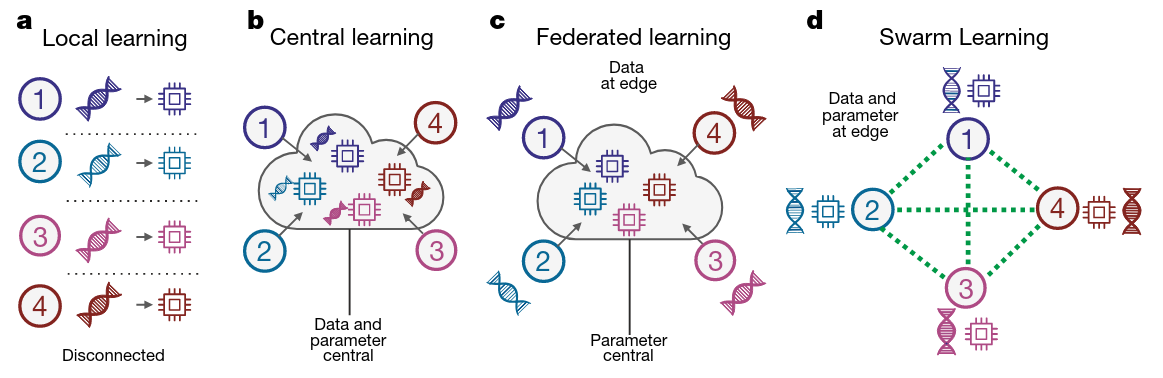
\includegraphics[width=\linewidth]{sl}
	\caption{Diagram of swarm learning compared to other type of learning taken from \cite{swarm_learning}}. The DNA icon denotes the location of data and the CPU icon denotes the location the model is stored
	\label{fig_learning}
\end{figure}


In SL, nodes learn in a similar fashion to FL in training steps. However, the nodes do not need to have their training steps synchronised. Following are the typical training steps of a swarm learning node:
\begin{enumerate}
	\item A node obtains a copy of the current model from the blockchain
	\item The node performs some training with their copy of the model and their own private data
	\item The updated model is merged with the latest blockchain model and sent back to the blockchain for other nodes to use
\end{enumerate}
The model on the blockchain will improve over time, and after a certain number of steps the blockchain model is the final output. \\

% Specify why swarm learning is better than conventional learning or federated learning
SL exhibits many of the same benefits of FL over conventional learning, but it also improves upon FL in some aspects. As is often the case when comparing decentralised algorithms to their centralised counterparts \cite{swarm_resil}, the absence of a central server makes SL more resilient to failures than centralized FL approaches such as FedAvg. The lack of a leader election protocol also means that SL may be better suited to tasks where networks of nodes are sparsely connected, as leader election in dynamic networks is a complex problem and can add large amounts of overhead \cite{leaderelection}. Additionally, the removal of the need for a server in SL reduces the likelihood of performance bottlenecks for very large swarms.

\section{Blockchain}
\todo{Write this out}

% Breif intro of what a blockcahin is
Blockchain is ... \cite{blockchain_review}

% Disadvantages of using blockchain
%% Scalability
Blockchain has problems with scalability \cite{blockchain_scale}.

%% High transaction cost
Blockchain is inefficient and slow \cite{blockchain_scale}.